\chapterimage{Dewatering.jpg} % Chapter heading image

\chapter{Theory Part II}

\section{Secondary Treatment}\index{Secondary Treatment}
\begin{itemize}
\item While preliminary and primary treatment processes are designed primarily to remove solids from wastewater, secondary treatment is for the removal of organics.
\item Secondary treatment involves:
\begin{itemize}
\item biological conversion of the dissolved and suspended organics in wastewater into biomass, and
\item physical settling (separation) process where the solids including the biomass formed during secondary treatment is separated and removed from the treated wastewater.
\end{itemize}

\item With the removal of gross solids in the preliminary treatment followed by removable of settleable solids in the primary clarifiers and the removal of dissolved and suspended organics in the secondary treatment processes, the wastewater is considered treated.
\item Secondary treated wastewater is typically disposed or treated further for reuse or disposal (depending upon the end use/application and the NPDES permit stipulations).
\item The solids (biomass) removed from the secondary treatment is typically mixed with the solids from primary treatment and stabilized using a solids treatment process like sludge digestion prior to its disposal.
\end{itemize}
\vspace{1cm}

\textbf{Secondary treatment process incorporates one of the following three approaches:}


\subsection{Fixed film system}\index{Fixed Film System}	
		
Trickling filter is a fixed film secondary treatment process wherein the organic content of the wastewater is removed using biological growth attached to an inert media such as lava rock or plastic\\
\begin{center}
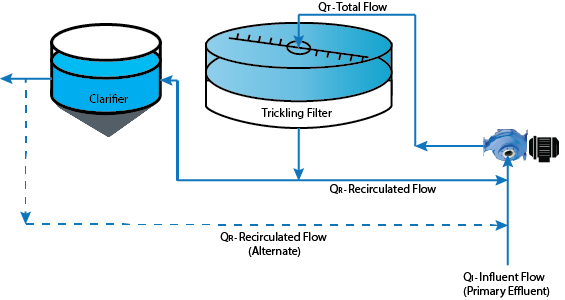
\includegraphics[scale=0.5]{TricklingFilter}
\end{center}		
\begin{itemize}
\item In a trickling filter, the wastewater is sprayed evenly on the surface of the media with a rotary type distributor with orifices
\item The wastewater percolates through the media bed, where it comes in contact with biological slime growth – zoogleal film (zooglea)
\item The aerobic biomass - bacteria, protozoa and other microoorganisms in the zooglea capture and consume the suspended and dissolved organics from the wastewater.
\item The microorganisms metabolize the organics and in the process produce more microbial mass resulting in increasing the thickness of the zoogleal layer.
\item The thickness of the zoogleal layer can only increase to a point until the wastewater flow – hydraulic load, shears the slime layer – “sloughs off” and is carried out as part of the effluent flow as sloughing.
\item The treated wastewater cascades from the bottom of the media into the underdrain system – lower portion of the TF comprised of columns which support the media base.  The underdrain has a sloping floor to direct the cascading water into a center channel .
\item The clarifier allows for the separation (settling) of the  of the solids (sloughed off material).  The settled solids is removed - typically pumped to a digester and the clarified effluent flows out of the clarifier.
\item The source of oxygen to support the aerobic growth is from the oxygen dissolved in the wastewater as it is sprayed over the media and from the air currents due to the downward flow of the wastewater and the temperature difference between ambient and the interior of the trickling filter.  Forced ventilation system may be designed as part of the trickling filter

\item Word trickling “filter” is a misnomer - no filtration is involved
\item Advantage includes process simplicity and lower costs
\item Disadvantage include BOD removal efficiency of only about 80-85%
\item The media may be rock, slag, coal, bricks, redwood blocks, molded plastic, or any other sound durable material.
\item The media depth ranges from about three to eight feet for rock media trickling filters and 15 to 30 feet for synthetic media.
\item The media needs to be uniformly sized and have adequate empty spaces (voids) to ensure maintaining aerobic condition necessary for the survival of biomass.  

\item Pre-fabricated (synthetic) media - similar to the one shown below, has an advantage over the "dumped" type media such as lava rock of providing a greater surface area per volume upon which the zoologeal film may grow while providing ample void space for the free circulation of air.

\item Sometimes, due to inadequate hydraulic loading, portions of the zoogleal layer may become too thick and oxygen cannot penetrate its full depth, causing odor issues.





\end{itemize}



\subsection{Suspended Growth System}\index{Suspended Growth System}
\begin{itemize}
\item In this type of secondary treatment, the microbes are suspended in the
wastewater flow being treated. 
\item Air or oxygen is supplied to maintain an aerobic environment and to keep the microorganisms in suspension. 
\item Example of this secondary treatment approach include the activated sludge treatment process 
\end{itemize}

\subsubsection{Elements of Activated Sludge Process}\index{Elements of Activated Sludge Process}

\begin{center}
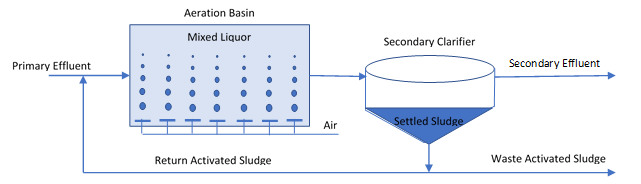
\includegraphics[height=4.5cm]{ASProcess}
\end{center}
\begin{itemize}

\item Utilizes an aeration basin/reactor and a secondary clarifier

\item In the presence of oxygen, aerobic bacteria in the aeration basin consume the organic matter (BOD) in wastewater for their growth and reproduction, converting BOD into bacterial cell mass along with metabolic byproducts including carbon dioxide and water

\item The aerobic bacteria is the predominant microbial life form in the aeration basin.  Other higher microbial life forms — mainly protozoa, are present along with some metazoans.

\item The microorganisms along with their metabolic byproducts and residual dead cell mass form a cluster called floc.

\item The wastewater exiting the aeration basin enters a clarifier where the floc settles.  The clear, treated secondary effluent flows out.

\item A portion of the settled activated sludge floc, is returned from the clarifier to the front of the aeration basin to seed the activated sludge treatment of the incoming primary effluent. The recycled floc is called \textbf{Return Activated Sludge (RAS)}.

\item The remaining settled floc from the clarifier is ”wasted” \textemdash transferred for solids treatment (typically using digestion) prior to its ultimate disposal. The wasted floc is called \textbf{Waste Activated Sludge (WAS)}.

\item The color of healthy activated sludge is tan to brown with an earthy/musty odor.

\item For activated sludge treatment to be effective, it is critical to establish a healthy microbial population which \hl{converts the BOD} into \hl{easily separable biomass.}
\item If the biomass does not settle well in the clarifier, it will be carried out in the treated secondary effluent producing a poor quality effluent with higher solids and organic content.  \\
\end{itemize}


\subsection{Pond System}\index{Pond System}
Similar to the suspended growth, stabilization ponds are large man made bodies of water which treat wastewater using mainly natural processes including sunlight, algae and microorganisms.
\begin{itemize}
\item Stabilization ponds and lagoons are bodies of water which treat wastewater using mainly natural processes including sunlight, algae and microorganisms for treating wastewater\\
\item While ponds are shallow and man-made, lagoons are bodies of water confined within natural boundaries.\\
\end{itemize}

 , which break down the effluent. It is in the anaerobic pond that the influent begins breaking down in the absence of oxygen "anaerobically". The anaerobic pond acts like an uncovered septic tank. Anaerobic bacteria break down the 

\subsubsection{Anaerobic Ponds}\index{Anaerobic Ponds}	

\begin{itemize}	
\item Typically for treating raw sewage
\item These are deep - 10-14 feet treatment ponds which rely primarily on anaerobic bacteria to break down the organic waste.
\item Designed for BOD removal
\item High strength wastewater may be treated.
\item Organic matter is broken down releasing releasing methane, carbon dioxide and odorous gases including hydrogen sulfide. 
\item Most of the decomposition is accomplished by acid forming bacteria. 
\item The pH in these lagoons is usually below 6.5. 
\item They are total retention and do not have an effluent discharge. 
\item The anaerobic pond must be de-sludged approximately once every 2 to 5 years
\item Organic loading of 200-1000 lbs. $BOD_5$ per acre per day
\end{itemize}

\subsubsection{Facultative Ponds}\index{Facultative Ponds}	

\begin{itemize}
\item The depth of facultative ponds is about 4-7 feet which is in-between the depths of anaerobic ponds (10-14 feet) and aerobic ponds 3 feet)
\item The uper layer of facultative pond is aerobic, and bottom layer is mostly anaerobic.
\item Facultative bacteria are responsible for most of the treatment that occurs in these ponds.  Facultative bacteria are bacteria which can live under both aerobic and anaerobic conditions.
\item The algae that grow in the pond are critical to the successful stabilization of the organic load. 
\item The algae will take in carbon dioxide ($CO_2$) and, through photosynthesis, use it to create sugars and release dissolved oxygen ($O_2$) that is used by the aerobic bacteria. Facultative lagoon levels should always maintain at least 4 feet of water in the pond.
\item Typically for secondary treatment - BOD removal
\item 15-50 lbs $BOD_5$ per acre per day.
\item Unused CO$_2$ will react with water to form carbonic acid - which would reduce the pH unless consumed
\item Sludge removal need is rare.  Sludge can be removed by using a raft-mounted sludge pump or by draining and dewatering the pond and removing the sludge with a front-end loader.
\end{itemize} 

				\begin{sidewaysfigure}
\begin{center}
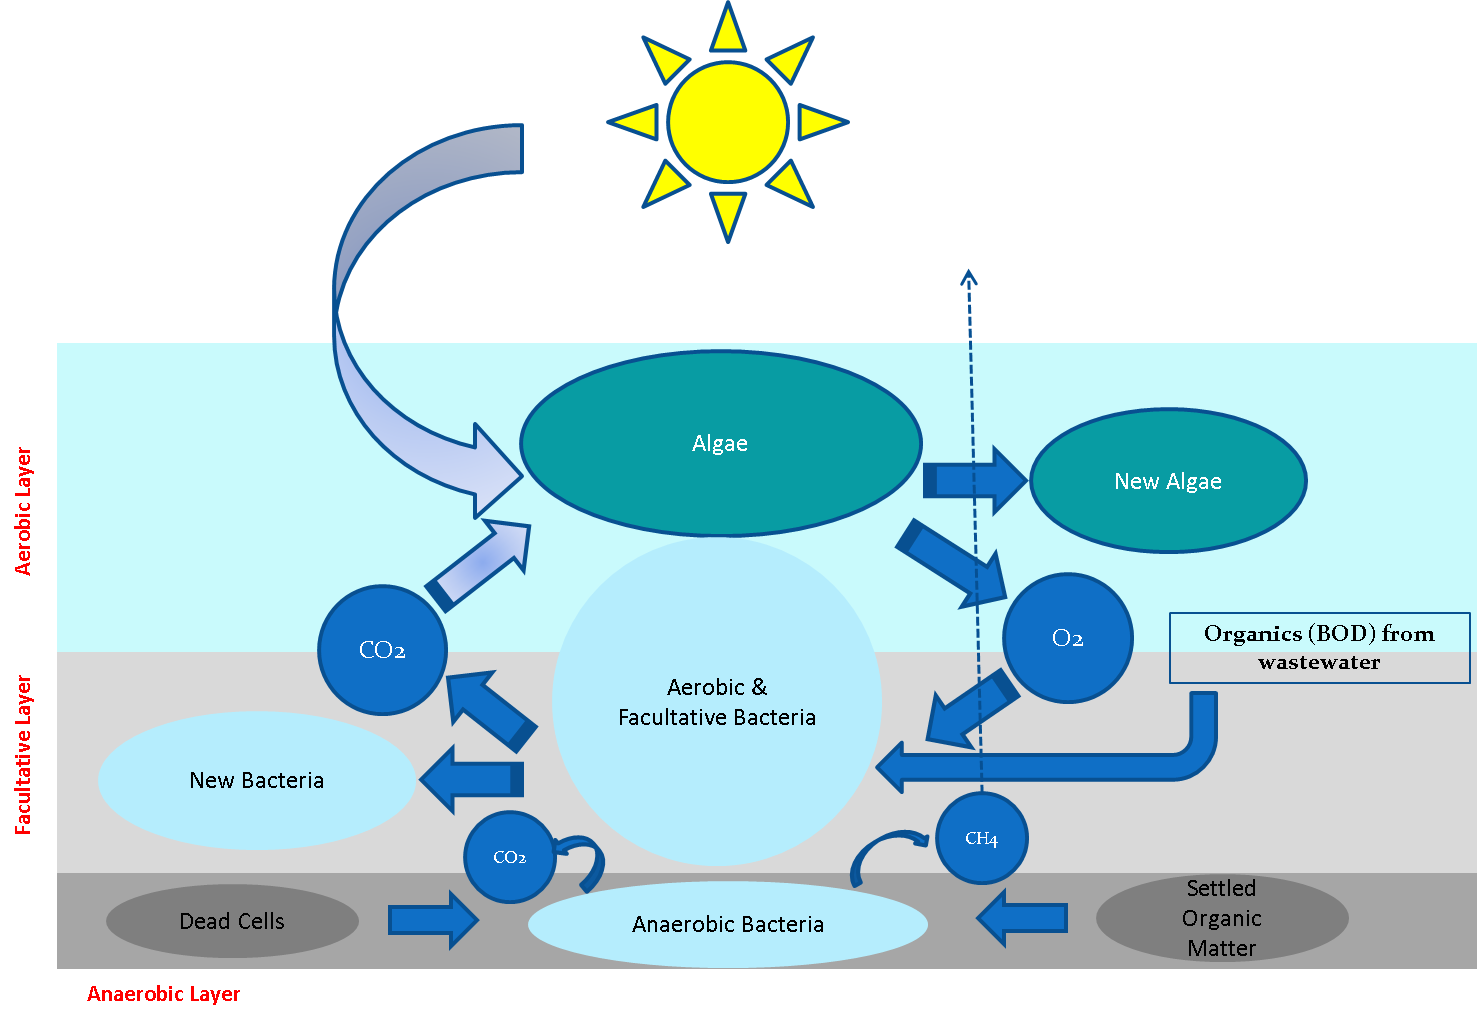
\includegraphics[scale=0.8]{StabilizationPond}\\
Facultative pond schematic
\end{center}
				\end{sidewaysfigure}
				
\subsubsection{Aerobic Stabilization Ponds}\index{Aerobic Stabilization Ponds}
	
Aerobic stabilization ponds are also known as: \hl{maturation}, \hl{polishing} or \hl{finishing} Pond
\begin{itemize}
\item Contain disssolved oxygen throughout entire depth of the pond.
\item Treatment is accomplished through the stabilization of organic wastes by aerobic bacteria and algae.
\item Typically for tertiary treatment
\item Designed for pathogen removal
\item Shallow - only about 3 feet deep. 
\item They are most often the final cells in a multi-staged pond system
\item They are also used as polishing ponds for tertiary treatment of trickling filter plant effluent.
\item Usually the effluent is directed into a second pond where the sludge can settle 
\item Their shallow depth allows sunlight to penetrate to the bottom of the pond to encourage algae growth and aerobic conditions throughout the pond 
\item The low solids loading found in these tertiary treatment applications means that these ponds normally have no sludge zone
\item These ponds may be mechanically aerated 
\item Aerobic polishing ponds are designed for 15-20 pounds BOD/acre/day
\item Aerobic ponds are typically designed for pathogen removal
\item Aerobic lagoon levels should always maintain at least 18 inches of water in the pond
\end{itemize}









\section{Solids Treatment}\index{Solids Treatment}




\subsection{Why do we need to treat wastewater solids?}\index{Why do we need to treat wastewater solids?}

\begin{itemize}
\item Sludge is generated from the wastewater treatment processes -  settled solids and scum from primary and secondary treatment processes
\item This sludge contain organic compounds and also elements that are beneficial plant nutrients
\item However, the organic solids in the sludge are not stable (i.e. they will decay) and include pathogens.  \item Prior to disposal, sludge has to be treated – stabilized, so that its disposal or reuse does not pose a threat to public health.
\item Sludge treatment is very critical as it is an expensive process and sludge disposal is subject to strict regulatory requirement.
\item Even solids are only a small component of wastewater, the solids treatment and disposal account for a very substantial portion of wastewater treatment costs.  Typically 40 to 60\% of total wastewater treatment operations cost is attributable to sludge treatment and disposal.
\end{itemize}

\textbf{NOTE: Solids removed during Preliminary Treatment, from barscreens and grit chambers are typically not treated as part of the solids treatment process.  These solids are disposed off at a landfill}

\vspace{0.5cm}
\textbf{Typical solids treatment is comprised of the following three sequential steps:
\begin{enumerate}
\item Sludge thickening
\item Sludge stabilization
\item Sludge dewatering
\end{enumerate}}
\vspace{0.5cm}

\subsection{Sludge thickening}\index{Sludge thickening}
Sludge thickening involves the removal of excess water from the primary and secondary sludge increasing the solids content of the sludge and reducing the volume of sludge to be treated in the sludge stabilization process.
Sludge thickening reduces the volume of sludge that need to be handled in the sludge stabilization step thereby reducing treatment cost.  
\begin{itemize}
\item There is an upper limit of the solids concentration that can be effectively treated (stabilized) as increasing the solids concentration reduces its ability to be mixed and pumped easily.  Typically the sludge thickening process produces sludge with a solids content of less than 10\%.\\
\end{itemize}
Benefits of thickening to the sludge stabilization process include:
\begin{itemize}
\item Improved performance due to a lower volume of sludge
\item Cost savings in the construction of new facilities
\item Reduction in energy requirements as less water has to be heated
\end{itemize}
Typical methods used for sludge thickening include:
\begin{enumerate}
\item Gravity thickener - more suitable for primary sludge
\item Dissolved air floatation thickener - more suitable for lighter, fluffier floc such as the secondary sludge.
\end{enumerate}
\subsection{Sludge Stabilization}\index{Sludge Stabilization}
\textbf{}\\
Sludge stabilization process produces solids that are deemed safe for eventual disposal.  Federal Part 503 rule establishes requirements for the final use or disposal of sewage sludge.  The solids disposal methods may include: land application, as a crop/vegetation fertilizer, placed on a surface disposal site for final disposal and fired in an incinerator.\\
\textbf{Biosolids is the term used for stabilized sludge which meets regulatory standards for beneficial reuse}\\  

Sludge stabilization process results in the following:
\begin{enumerate}
\item Reduction in amount of solids
\item Pathogen reduction
\item Odor reduction
\item Reduction in vector attraction
\end{enumerate}
The main processes involved in sludge stabilization include:
\begin{itemize}
\item Digestion - Aerobic or anaerobic
\item Lime or alkaline stabilization
\item Composting
\item Long term storage in lagoons
\item Thermal processes
\item Incineration
\end{itemize}

Most common processes involved in sludge stabilization include:

		\begin{enumerate}
		\item Digestion - Aerobic or anaerobic
		\item Lime or alkaline stabilization
		\item Composting
		\item Long term storage in lagoons
		\item Thermal processes
		\item Incineration
		\end{enumerate}
		\begin{itemize}
		\item \hl{Sludge digestion is a microbiological process and is the most common sludge stabilization method}.
		\item There are two major sludge digestion processes:
			\begin{itemize}
			\item aerobic digestion which utilizes aerobic microorganisms, and produces carbon dioxide as a byproduct
			\item anaerobic digestion which utilizes anaerobic microorganisms and it produces digester gas as a byproduct.
			\item Digester gas is typically composed of 60-65\% methane gas with the remainder being mostly carbon dioxide ($CO_2$) and is useful because of its potential use as fuel - energy recovery from wastewater.
			\end{itemize}
		\end{itemize}

\subsection{Sludge Dewatering}\index{Sludge Dewatering}
Solids stabilized using digestion process has only a small percentage by weight of solids -less than 5\%.  It therefore becomes necessary to dewater the stabilized sludge prior to hauling off-site for final disposal.  Like thickening, the dewatering process does not treat the sludge.  It increases the solids content to between 15 to 30 percent and the higher solids content of the stabilized sludge makes it easier to handle and reduces costs associated with elements related to accomplishing the end objectives with the sludge – land application, composting, drying, incineration or landfill.\\
Dewatering involves conditioning the sludge with a polymer and subjecting it to a physical process which include:
\begin{enumerate}
\item Belt Filter Press 
\item Centrifuge
\end{enumerate}
\newpage
\section{Anaerobic Digestion}\index{Anaerobic Digestion}
			\begin{itemize}
			\item \hl{Anaerobic sludge digestion is a microbiological process and is the most common sludge stabilization method}
			\item anaerobic digestion utilizes anaerobic microorganisms and produces digester gas as a byproduct.
			\item Digester gas is typically composed of 60-65\% methane gas with the remainder being mostly carbon dioxide ($CO_2$) and is useful because of its potential use as fuel - energy recovery from wastewater.
		\item Solids removed from the primary and secondary treatment processes is fed to the digesters.  
		\item The sludge feed to the digesters range between 3 – 6\% total solids which typically contain 70\% organic solids
		\item The anaerobic digester is typically a large cylindrical concrete tank and is operated as a continuous process at a fixed volume\\ $\implies$ as sludge is fed into the digester it displaces an equal amount of sludge which leaves the digester.
\begin{center}
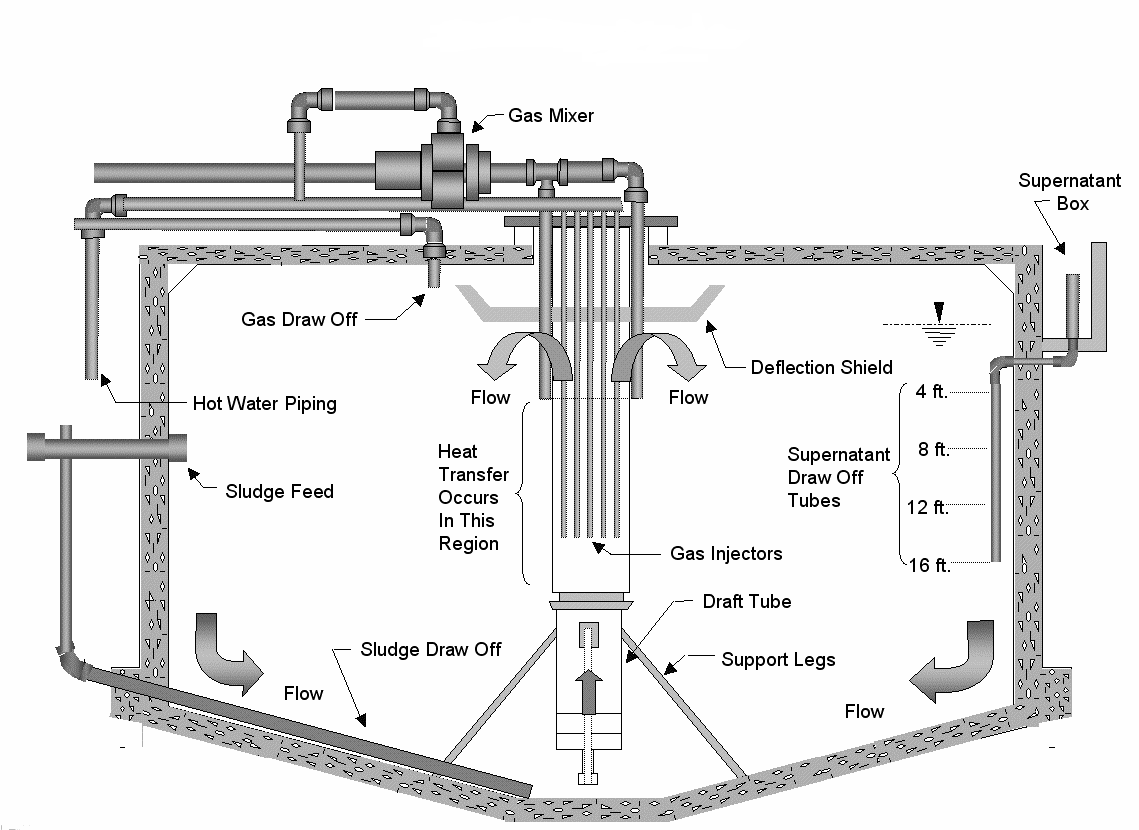
\includegraphics[scale=0.50]{DigesterFixedCover}\\
\textbf{Anaerobic Digester}\\
\end{center}
		\item The sludge typically occupies 70 - 90\% of the total digester volume and the methane carbon dioxide gas mixture occupies the headspace from where it is withdrawn also on a continuous basis.
		\item In the anaerobic digestion process microorganisms convert volatile matter into mainly methane (CH$_4$) and carbon dioxide (CO$_2$)
		\item The sludge content of the digesters is kept mixed and maintained in a constant temperature range using external heating.
		\item The activity and type of bacteria present in the digester is dictated by the operating temperature of the digester.
		\item Anaerobic digestion can be in the following three temperature ranges, each of which has its own unique microbiology.\\
			\begin{enumerate}[1. ]
			\item Psychrophilic digester:  Digester is maintained between 50  - 65 F.  Sludge detention time - 50 to 180 days
			\item Mesophilic digesters: – Digester is most commonly operated  between 95 – 98 F and the typical number of days required for digestion is between 15 to 30 days.\\
			\item Thermophilic digesters:  These digesters’ optimal operating temperatures range is between 113   135 F and it typically requires 5 to 12 days.\\
			\end{enumerate}     
		\item These organic solids are measured as volatile solids (VS).  
		\item The volatile solids content of the sludge entering and leaving the digester are measured to quantify the solids removal in the digester
		 \item Breakdown of volatile matter in the sludge ultimately into methane (CH$_4$) and carbon dioxide (CO$_2$) occurs in multiple steps involving different groups of microorganisms as follows:\\
			\begin{enumerate}[Step 1.]
			\item Hydrolysis:  Here the microorganisms breakdown complex organic matter in the sludge - carbohydrates, proteins, lignin, and lipids into simpler compounds including sugars, soluble fatty acids and amines.\\
			\item Acid Formation:  The simpler compounds formed in Step 1 are converted to organic acids by acid forming bacteria\\
			\item Methane Formation: The organic acids formed in Step 2 are converted into methane and carbon dioxide by methane forming bacteria.\\
			\end{enumerate}
		\item Gas production ranges between 10 to 16 cubic feet per pound of volatile matter destroyed and the gas production remains stable over time.
		\item Low gas production indicates problems - toxicity, temperature, volatile acid to alkalinity ratio, mixing, or feed rates.
		\end{itemize}

\newpage
\section{Chlorination}


\begin{itemize}
\item Treated wastewater effluent is disinfected prior to its discharge into a water body inorder to destroy pathogens primarily to prevent spread of waterborne disease and minimize public health problems
\item Chlorine is a very effective disinfectant and is the most widely used disinfectant for wastewater 
\item Chlorine disinfection is a practical and economical means for disinfecting large quantities of wastewaters which have been treated to various degrees. 
\item However, due to its toxicity, associated risk factors and its rising cost, use of ultraviolet light and ozone for wastewater disinfection is on the rise
\end{itemize}


\subsection{Forms of Chlorine}\index{Forms of Chlorine}

\begin{itemize}
	\item Due to safety issues related to the use of chlorine gas, 			\textbf{hypochlorites} are often used in lieu of chlorine
	\item Types of hypochlorites
	\begin{itemize}
	\item Sodium hypochlorite (NaOCl) comes in a liquid form which contains up to 12.5\% chlorine
	\item Calcium hypochlorite (Ca(OCl)$_2$), also known as HTH, is a solid which is mixed with water to form a hypochlorite solution. Calcium hypochlorite is 65-70\% concentrated.
	\end{itemize}
	\item Hypochlorites decompose in strength over time while in storage. Temperature, light, and physical energy can all break down hypochlorites before they are able to react with pathogens in water. 

\end{itemize} 

\subsection{Chlorine Properties}\index{Chlorine Properties}

\begin{itemize}
\item Chlorine is a yellowish-green gas at room temperature and atmosphric pressure
\item Chlorine gas can be pressurized and cooled to its liquid form for making it easy to ship and store. 
\item When liquid chlorine is released, it quickly turns into a gas that stays close to the ground (being heavier than air) and spreads rapidly.
	\item 	While it is not explosive or flammable, as a liquid or gas it can react violently with many substances 
	\item Chlorine is only slightly soluble in water (0.3 to 0.7\% by weight.) 
	\item Chlorine gas has a greenish-yellow color 
	\item It has a characteristic disagreeable and pungent odor, similar to chlorine-based laundry bleaches, and is detectable by smell at concentrations as low as 0.2 to 0.4 ppm
	\item It is about two and a half times as heavy as air
	\item One volume of liquid chlorine yields about 460 volumes of chlorine gas. 
	\item Liquid chlorine is amber in color and is about one and a half times as heavy as water 
	\item Chlorine is an irritant to the eyes, skin, mucous membranes, and the respiratory system 
\end{itemize}


\subsection{Chlorine Storage and Safety}\index{Chlorine Storage and Safety}


\subsubsection{Chlorine Delivery}\index{Chlorine Delivery}

\begin{itemize}
\item Typically for smaller plants chlorine gas is shipped in  pressurized steel cylinders - 150 lb or 2000 lb (ton cylinder) size
\item Larger plants may get their chlorine supply in rail tank cars
\item The daily chlorine usage is typically established based upon the weighing of the chlorine containers.
\end{itemize}


\subsubsection{Chlorine Leak Response}\index{Chlorine Leak Response}
\begin{itemize}
	\item Typically for smaller plants chlorine gas is shipped in  pressurized steel cylinders - 150 lb or 2000 lb (ton cylinder) size.  Larger plants may get their chlorine supply in rail tank cars.  
	\item The daily chlorine usage is typically established based upon the weighing of the chlorine containers.
	\item The withdrawal rates from a chlorine cylinder is based on the temperature of the liquid in the cylinder, and thus the pressure of the gas. 
	\item As chlorine gas is withdrawn from the cylinder, it absorbs the heat from the surroundings.
	\item For low withdrawal rates, heat will be able to be transferred from the surrounding air to the container in time so that there is no drop in temperature or pressure, 
	\item If the chlorine withdrawal is larger, the air will not be able to transfer the heat quickly enough and the temperature (and pressure) of the chlorine will drop, thus resulting in a lower feed rate. 
	\item If high enough and prolonged enough, this can even result in ice formation around the outside of the container, further decreasing the withdrawal rate. 
	\item The most effective way to increase withdrawal rate from a single container is to circulate the surrounding air with a fan. Again, never apply heat to the containers.
	\item If chlorine gas escapes from a container or system, being heavier than air, it will seek the lowest level in the building or area
	\item Only trained staff with access to proper personal protection equipment (PPE) including self-contained breathing apparatus, should handle the chlorine cylinders and address chlorine leak issues 
	\item When a leak is suspected, it is recommended that ammonia vapors be used to find the source. When ammonia vapor using a rag or brush, is directed at a leak, a white cloud will form. To produce ammonia vapor, a plastic squeeze bottle containing about 5 \% ammonia, aqua ammonia (ammonium hydroxide solution) should be used. A weaker solution such as household ammonia may not be concentrated enough to detect minor leaks
	\item All safety equipment should be located outside of the chlorine room and be easily accessed by all personnel
	\item Small leaks around valve stems can usually be corrected by tightening the packing nut or closing the valve. A leak can also be reduced by removing the chlorine as rapidly as possible
	\item If it cannot be added to the process there are several chemicals which can be used to absorb the chlorine gas. For example, chlorine can be absorbed by using 1$frac{1}{4}$ pounds of caustic soda or hydrated line, or 3 pounds of soda ash per pound of chlorine. 
	\item If the leaking container can be moved, it should be transported to an outdoors area where minimal harm will occur. Keep the leaking part the most elevated so that gaseous chlorine will leak rather than liquid chlorine.
	\item If the leak is large, all persons in the adjacent area must be warned and evacuated. Only authorized persons equipped with the proper breathing apparatus, and protective measures to the eyes and body should investigate. 
	\item As water is not an efficient absorbent for chlorine and the fact that chlorine reacts with water to form very corrosive hydrochloric acid, never apply water to a leak or consider submerging a chlorine cylinder (for example, in a pond or tank), since it will probably float.
	\item Remember to keep windward of the leak.
	\item As chlorine cylinders pressure increases with temperature, as a safety measure the chlorine cylinders are fitted with fusible plug which melts between 158$^o$ and 165$^o$ F.
	\item Keep chlorine cylinder or container emergency repair kits available. Be familiar with their use and location.
	\item Leaks at fusible plugs and cylinder valves requires special handling and emergency equipment. The chlorine supplier must be notified immediately
	\item Pin hole leaks in cylinder walls or ton tanks can usually be stopped by mechanical pressure applications (clamps, turnbuckles, etc.). This only temporary and may require your ingenuity.
	\item Leaking containers cannot be shipped.
	\item In general, daily inspection of all chlorine cylinders will avoid major problems
\end{itemize}

\subsubsection{Chlorine Reactions Related to Disinfection}\index{Chlorine Reactions Related to Disinfection}
\textbf{Chlorine reacts with water to form hypochlorous and hydrochloric acids}\\
Cl$_2$ \hspace{0.8cm}	+ \hspace{0.3 cm}	 H$_2$O		\hspace{0.8cm} $\iff$ 
\hspace{0.8cm} HOCl	\hspace{0.8cm}	 +	\hspace{0.8cm}	 HCl \\
chlorine \hspace{0.8cm}	water \hspace{1.8cm}		 hypochlorous acid	\hspace{0.1cm}	 hydrochloric acid\\ 
	\vspace{0.5cm}
	\begin{itemize}
		\item Hypochlorous acid dissociates in water to form the hydrogen and hypochlorite ions\\
 HOCl \hspace{1.8 cm} $\iff$ \hspace{1.8 cm} H$^+$ \hspace{1.8cm} + 	\hspace{0.8cm}OCl$^-$\\ 
hypochlorous acid  \hspace{1.9 cm}      hydrogen ion   \hspace{1.5cm}           hypochlorite ion

		\begin{itemize}
			\item Hypochlorous acid is the most effective form of chlorine available to kill microorganisms
			\item Hypochlorite ions is much less efficient disinfectant
		\end{itemize}

		\item The concentration of hypochlorous acid and hypochlorite ions in chlorinated water will depend on the water's pH
		\begin{itemize}
			\item A higher pH facilitates the formation of more hypochlorite ions and results in less hypochlorous acid in the water
		\end{itemize}
		\item A significant percentage of the chlorine is still in the form of hypochlorous acid even between pH 8 and pH 9
		\end{itemize}



\subsection{Chlorine Disinfection}\index{Chlorine Disinfection}

\begin{itemize}
\item When chlorine is added to a wastewater flow, it will first react or combine with certain organic and inorganic substances present, prior to acting on pathogens.  The amount of chlorine used up as part of these reactions is referred to as the \textbf{chlorine demand}\\

\item The \textbf{free chlorine} remaining after the chlorine demand is satisfied, is the strongest form of chlorine available for disinfection.  

\item Chlorine combined with ammonia (as chloramines) and organic compounds (as chloroorganic compounds), known as \textbf{combined chlorine} also exhibit disinfecting properties - albeit weaker than the free chlorine.

\item \text{Total residual chlorine} is the sum of free chlorine and combined chlorine and it is the residual chlorine concentration which represents the amount of chlorine available for disinfection 

\item \textbf{Chlorine Demand = Applied Chlorine Dose - Chlorine Residual}\\ Chlorine residual should be the basis of measuring the effectiveness of chlorine disinfection

\item Chlorine residuals are measured in the field using a colorimeteric method.  In the laboratory, chlorine residuals are measured typically using: 1) Amperometric Titration, or 2) Iodometric Titration

\item Chlorine dosage is typically established from either bench scale laboratory testing, or actual measurement of field results. 

\item Since field conditions, particularly the mixing element, are not as well controlled as laboratory tests, the actual dosage is expected to be generally higher than from that established in the laboratory. 

\item Even though residual chlorine concentration can be used for establishing the effectiveness of disinfection, the ultimate effectiveness of disinfection can be monitored by conducting bacteriological testing.

\end{itemize}

\subsection{Factors Affecting Chlorine Disinfection Efficiency}\index{Factors Affecting Chlorine Disinfection Efficiency}

The disinfection efficiency of chlorine depends on the following factors:\\
\begin{itemize}
	\item pH:  Disinfection is more efficient at a low pH when large quantities of hypochlorous acid are present than at a high pH when hypochlorite ions is the dominant species in the water
	\item Concentration:  Contact Time Ratio (CT):  For effective chlorine disinfection both sufficient chlorine dosages – concentration (C) as well as contact time (T) are necessary.  There may be a substantial residual but if CT factor is not adequate, disinfection may not be effective. Generally both of these factors must be worked out experimentally for a given system
	\item Temperature:  Colder temperatures are less favorable for disinfection. 
Proper contacting or mixing or agitation:  This is necessary to make sure that the chlorine applied contacts or reaches the microbial cells
	\item Organic and inorganic material present:  The chlorine used by these organic and inorganic reducing substances including metal ions, organic matter and ammonia, is defined as the chlorine demand.  So that the amount of chlorine that has to be added to wastewater for different purposes will also vary.
\item Even though residual chlorine concentration can be used for establishing the effectiveness of disinfection, the ultimate effectiveness of disinfection can be monitored by conducting bacteriological testing.
\end{itemize}
		
\subsection{Dechlorination}\index{Dechlorination}
\begin{itemize}
\item Dechlorination is the process of removing residual chlorine from disinfected wastewater prior to discharge into the environment
\item Dehlorination is necessary to mitigate the toxic effect of chlorine on the receiving waters.  
\item Sulfur dioxide is most commonly used for dechlorination.
\item Other chemicals used for sodium bisulfite, sodium sulfite and sodium thiosulfate.
\end{itemize}

\newpage

\section{Wastewater Treatment Hazards}\index{Wastewater Treatment Hazards}
There are many hazards encountered in wastewater treatment operations.  The hazards and their respective mitigation measures are as follows:\\
\subsection{Hazardous Chemicals}\index{Hazardous Chemicals}
\begin{itemize}
\item Hazardous chemicals are used throughout wastewater treatment plants and in collection systems. 
\item To understand the dangers of these chemicals and to take adequate steps OSHA requires that the chemical manufacturer, distributor, or importer provide Safety Data Sheets (SDSs) (formerly MSDSs or Material Safety Data Sheets) for each hazardous chemical to downstream users to communicate information on hazards related to that particular chemical or product.
\item Employers must ensure that the SDSs are available and readily accessible to employees for all hazardous chemicals in their workplace.
\item The SDS includes information such as the properties of each chemical; the physical, health, and environmental health hazards; protective measures; and safety precautions for handling, storing, and transporting the chemical.\\
\end{itemize}
\subsection{Hazardous Gasses}\index{Hazardous Gasses}
\begin{itemize}
\item A summary of the properties and effects of hazardous gases found in wastewater operations is provided in the table below.
\item To safeguard against the potential impacts of these gases, employees are required to follow practices including donning appropriate Personal Protective Equipment (PPE) and utilizing respiratory protection\\
\end{itemize}
\begin{center}
\includegraphics[scale=0.6]{SafetyHazardousGases4}\\ 
\end{center}

\subsection{Falls}\index{Falls}
\begin{itemize}
\item Falls are one of the leading causes of injuries and deaths on the job.  Fall protection is a combination of methods and devices used to protect workers from falling off, onto, or through working levels. 
\item Fall protection methods and devices are typically divided into two categories: those that prevent falls and those that arrest falls. 
\item Examples of fall protection methods and devices include rails, guards, guardrails, barriers, fall-arrest systems, safety nets, hole covers, and various work practices and procedures.
\end{itemize}
\begin{center}
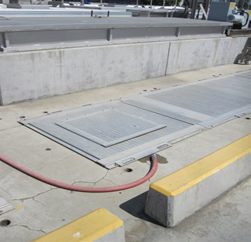
\includegraphics[scale=0.8]{SafetyFallProtection1}\hspace{1cm} 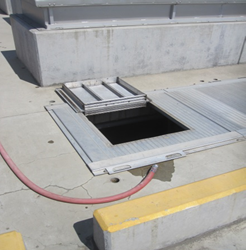
\includegraphics[scale=0.8]{SafetyFallProtection2}\\
\end{center}
\subsection{Noise}\index{Noise}
\begin{itemize}
\item Noise as a hazard is sound that is especially loud or impacting. 
\item A wastewater treatment plant has equipment that produces high noise levels both continuously and intermittently. 
\item As such, it is important to be aware of this hazard and to take preventive steps to reduce exposure to damaging noise levels by wearing effective hearing protection and to minimize the duration of the exposure to the noise.
\end{itemize}

\subsection{Electrical Hazards}\index{Electrical Hazards}
\begin{itemize}
\item Ordinary 120-V electricity can be fatal; most wastewater facility electrical systems operate at 120 to 4000 V or more.  
\item All voltages should be considered dangerous and potentially life threatening.  
\item Safe working rules and practices that should be followed when working on electrical systems
\item Before working on an electrical system, perform a job hazard analysis to determine any potential hazards and methods of abating those hazards
\end{itemize}


\subsection{Rotating and Moving Equipment}\index{Rotating and Moving Equipment}

\begin{itemize}
\item All rotating and moving equipment should be guarded. 
\item The best method for preventing machinery-related injuries is through use of equipment guards enforced through engineering and administrative controls.   
\item The best way to prevent this type of injury is to install point-of-operation guards that prevent contact with ingoing nip points, pinch points, rotating parts, flying chips, and sparks.
\end{itemize}
\begin{center}
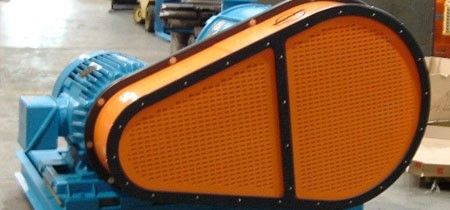
\includegraphics[scale=0.6]{SafetyMachineGuarding}\\
\end{center}

\subsection{Heat Stress}\index{Heat Stress}
\begin{itemize}
\item Heat stress falls into two categories: heat illness and heat stroke. 
\item Both are serious conditions and should not be taken lightly. 
\item Heat stress can result from: 
\begin{itemize}
\item High temperature and humidity, dehydration from low fluid consumption
\item Direct sun exposure (with no shade) or extreme heat, 
\item Limited air movement (no breeze or wind), 
\item Physical exertion, Use of bulky protective clothing and equipment, 
\item Poor physical condition or ongoing health problems, 
\item Some medications
\item Pregnancy
\end{itemize}
\end{itemize} 


\subsection{Safety Practices}\index{Safety Practices}
\subsubsection{Lockout - Tagout (LOTO)}\index{Lockout - Tagout (LOTO)}

When conducting routine inspections, repairs and maintenance activities, requires meeting the mandates of \hl{Occupational Safety  Hazard Administration(OSHAs) Lock-Out/Tag-Out (LOTO) program}\\
which is designed to prevent injury or fatalities.  It involves preventing an equipment from accidentally starting up and release of all stored energy.  Hazardous energy sources include: 
\begin{itemize}
\item Electrical 
\item Mechanical
\item Hydraulic
\item Pneumatic 
\item Chemical 
\item Thermal  
\item Other energy
\end{itemize}

The LOTO involves established and documented procedures specific to an equipment or machinery.  It typically comprises of:\\
\begin{itemize}
\item Notifying affected employees
\item Stopping and isolating the equipment
\item Releasing stored energy
\item Verification of the isolation and de-energization
\item Placing lock-out devices which use a positive means such as a lock, either key or combination type, to hold an energy isolating device in the safe position and prevent the energizing of a machine or equipment
\item Appropriately tagging the devices to indicate its non-operation and that it may not be operated until the tagout device is removed
\end{itemize}

\subsubsection{Personal Protective Equipment (PPE)}\index{Personal Protective Equipment (PPE)}
Employees depend on personal protective equipment to protect themselves from hazards and perform daily duties. PPE includes but is not limited to safety glasses, face shields, hard hats, gloves, foot protection, and durable and disposable chemical-protective clothing. Respirators and fall protection might also be required. However, respirators and fall protection fall under separate OSHA standards. \\

\subsubsection{Confined Space Entry}\index{Confined Space Entry}
OSHA defines a confined space as an area that:
\begin{itemize} 
\item is large enough and so configured that an employee's body can enter and perform assigned work
\item has limited or restricted means for entry or exit; and
\item is not designed for continuous employee occupancy.
\end{itemize}
A permit-required confined space is defined as a confined space that:
\begin{itemize} 
\item contains or has a potential to contain a hazardous atmosphere
\item contains a material that potentially could engulf an entrant
\item has an internal configuration that could trap or asphyxiate an entrant through inwardly converging walls or a floor that slopes downward and tapers to a smaller cross-section
\item contains any serious safety or health hazard
\end{itemize}

Potentially dangerous atmospheric conditions which can exist in confined spaces include: 
\begin{itemize}
\item Oxygen level: Some gasses are heavier than air and so will fill up a confined space, which forces oxygen out.  The oxygen concentration must not fall below 19.5\% at any time.  In plants where pure oxygen is used there is a potential hazard due to high the oxygen concentration.  Oxygen concentration greater than 23\% increases the risk of ignition and fire
\item Explosive conditions:  Many gasses are explosive when present in certain ratios with oxygen. These ratios are defined by the upper explosive limit(UEL) and the lower explosive limit (LEL).  The minimum concentration of a particular combustible gas or vapor necessary to support its combustion in air is defined as the Lower Explosive Limit (LEL) for that gas. Below this level, the mixture is too “lean” to burn. The maximum concentration of a gas
or vapor that will burn in air is defined as the Upper Explosive Limit (UEL). Above this level, the mixture is too “rich” to burn.  The range between the LEL and UEL is known as the flammable range for that gas or vapor.  
\item Toxic conditions:  This condition could potentially exist due to the presence of gasses such as carbon dioxide, chlorine and hydrogen sulfide.  
\end{itemize}